\documentclass[11pt, oneside]{article}   	% use "amsart" instead of "article" for AMSLaTeX format
\usepackage{geometry}                		% See geometry.pdf to learn the layout options. There are lots.
\geometry{letterpaper}                   		% ... or a4paper or a5paper or ... 
%\geometry{landscape}                		% Activate for for rotated page geometry
%\usepackage[parfill]{parskip}    		% Activate to begin paragraphs with an empty line rather than an indent
\usepackage{graphicx}				% Use pdf, png, jpg, or eps§ with pdflatex; use eps in DVI mode
								% TeX will automatically convert eps --> pdf in pdflatex		
\usepackage{amssymb}

\title{LHC Report}
\author{Canay Oz\\Gamze Sokmen \\ Gokcenur Yesilyurt}

%\date{}							% Activate to display a given date or no date

\begin{document}
\maketitle
%\section{}
%\subsection{}

\section{Introduction}

The LHC breaks big groups of protons into pieces at close to the speed of light. Some of these pieces have head on collisions and very energetic. When this happens some of the energy of the collision is turned into mass and previously unobserved, short-lived particles.
To achieve this, there are four main detectors; ATLAS, CMS, ALICE, LHCb. Two of them are general-purposed; ATLAS and CMS. In this report, we will point CMS up.
\\\\
The Compact Muon Solenoid (CMS) with the diameter is 15 m, the length is 21.5 m, is designed to detect and measure the sub atomic particles released during collisions. A part of the detector is inside in a giant solenoid magnet that can create a magnetic field nearly 100,000 times stronger than the Earth's magnetic field. 
The choice of the magnet field configuration for the measurement of the momentum of muons is an important point in the design of the detector. Momenta of high-energy charged particle is measured precisely with the help of large bending power. Hence, the superconducting technology for the magnets becomes essential. A 13 m long, 6 m inner diameter,
4 T superconducting solenoid is designed to provide this power. It can be seen as just the outside of the blue part from the Figure 1. 
\begin{figure}[H]
\begin{center}
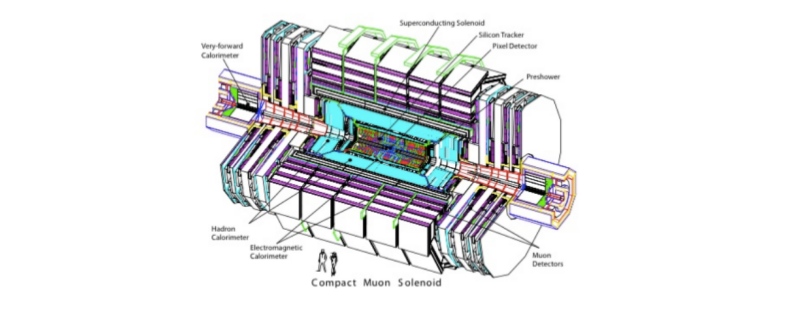
\includegraphics[width=13cm]{a1.png}
\end{center}
\caption{Compact Muon Solenoid }
\end{figure}

\\\\
Furthermore, there are many reasons for why the detector is so big. Firstly, the events create excessive amounts of energy, so the paths of particles
become very long. In order to absorb a far amount of them, sufficient amounts of materials are required. Second, the accuracy of measurements in momentum
depends on the size of the detector directly. If the travelled magnetic field is as big as enough, the bending of momentum becomes less, evenly.
Third, the strong magnetic field with 4 T, that is mentioned above, is used to bend the trajectories of charged particles as much as possible. To help this, there is an iron
return yoke (Figure 2.) in the detector as the biggest part with 12 500 tones. As a result of all of this, CMS is 15 metres in diameter and weighs around
the same as 2,500 African elephants.
\begin{figure}[H]
\begin{center}
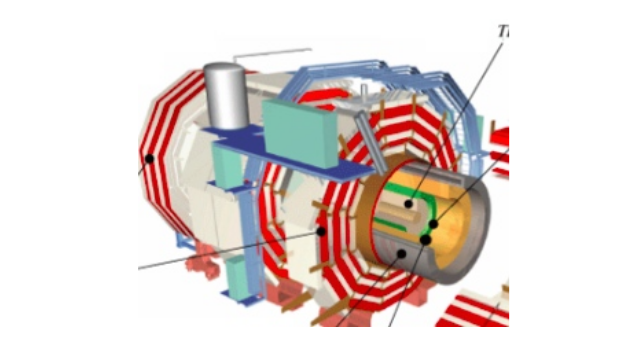
\includegraphics[width=7cm]{a2.png}
\end{center}
\caption{Iron Yoke}
\end{figure}




CMS detector is similar to a hypothetical cylindrical onion that has many layers to stop, track or measure a different type
of particle emerging from collisions. Finding the energy and momentum of a particle gives clues to its identity, and particular
patterns of particles. 

\begin{figure}[H]
\begin{center}
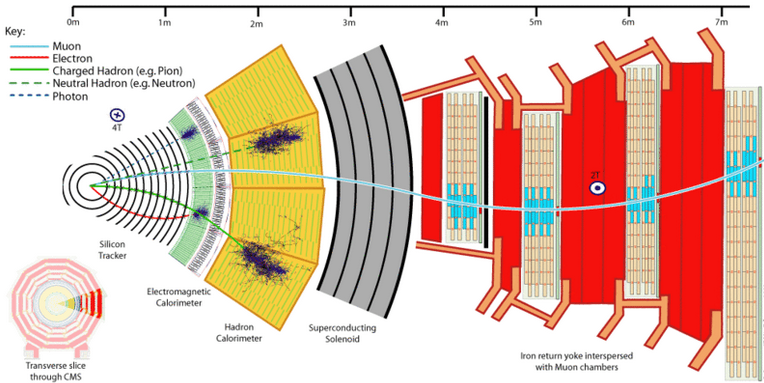
\includegraphics[width=10cm]{r3.png}
\end{center}
\caption{Compact Muon Solenoid }
\end{figure}

\section{Tracker}

First layer of the onion is the tracker which is made of silicon. Tracker has been made to mainly measure particles momentum. For this purpose tracker should interfere with particles
as little as possible. One method to calculate the momentum of a particle is to track its path through a magnetic field. CMS tracker records the paths taken by charged particles 
at a number of key points and then reconstruct paths from that key points.

Measurement must be very accurate, every measurement of tracker is accurate to 10 micrometer. 
It is also the inner most layer of detector. Because of this, construction materials were carefully chosen to resist radiation. It is very interesting that in the very 
first design sketch of CMS, tracker section was blank because it was thought that it would be impossible to make a tracker that could withstand to the intensity of particles.
Tracker consists of pixels and silicon microstrip detectors. Pixels are at the very core of detector and dealing with highest intensity of particles where silicon strips surround pixels. 
The pixel detector, though about the size of a shoebox, contains 65million pixels which allows it to track the paths of particles with extreme accuracy. This accuracy is needed because there 
are 10 million particle per square centimetre per second. Each silicon sensor is 100 micrometer by 150 micrometer. When a charged particle passes through on of this sensors a small electric current
observed due to ejected electrons from silicon atoms. A electronic silicon chip used to amplify the signal. Knowing which pixels touched allows us to deduce particle`s trajectory.
After pixels, particles pass through ten layers of silicon strip which are reaching out to 130 centimetres. There are 10 million detectors strips which read by 80000 microelectronic chips.
Silicon strips work in much the same way as the pixels with fast response and good spatial resolution. To minimise disorder due to high radiation silicon strips freeze to -20 C. Much of the
technology behind tracker electronics came from innovation in collaboration with industry.
\section{Electromagnetic Calorimeter}
In order to build up a picture of events CMS must find the energies of particles. In order to achieve this CMS uses electromagnetic calorimeter (ECAL). ECAL must be fast with high precision. 
Lead tungstate crystal is made for this purpose which is heavier than stainless steel but with a touch of oxygen in crystalline form it is transparent and produce light when particles
pass through. The light produced by this crystal is proportional with particle`s energy. To detect this light, photodetectors are glued onto the back of each of the crystals. ECAL is made up of a barrel
and two end caps. Barrel consists of 36 super modules which have total of 61200 crystals. Each crystal weigh 1.5 kg with a total of 78000 crystals weigh around 120 tons. It took about ten years to grow
all 78000 crystals. It takes two days to artificially grow each crystal.

\section{Hadron Calorimeter}

After mentioning in the order; tracker 
and electromagnetic calorimeter now we can talk about hadron calorimeter
part of the CMS which is the detector has the world's largest superconducting magnet. Hadronic calorimeter was built to measure the energy of mainly hadrons
which are also named as mesons and baryons (particles constructed with qurks and gluons). This part of the CMS is important also for the indirect measurements
of non-interacting uncharged neutrinos. The reason beyond the importance of this measurements is to learn more about the Higgs Boson and also for the search
on new physics theories such as SUSY (Supersymmetry), which can be approaced as the most common accepted beyond The Standard model theory in today's particle
physics world. Since in this part of the detector we are searching for the heavier particles, we should know the fact that they can decay very fastly and in
other words, they do not leave the record of their presence in any other parts of the CMS except the HCAL (hadronic calorimeter) part to detect them.
As a physical feature, it was decided during the constuction of the CMS, it was better for the HCAL has a hermetic shape which means it should have a large solid
angle coverage to observe as many as particle's energy. In the case of an imbalance situation in the energy, these particles can be shoot out from one side of
the detector but not the other, therefore it better to do measurements with the transverse momentum (the momentum not through the beam line, the momentum perpendicular to
beam line). Then it can be said that for these kind of measurement, we are dealing with invisible particles.
\\\\
It is also known that there are no gaps which particles can escape through them in the HCAL. With this feature, we increase the probability of seeing new physics.
For HCAL, it can be also said it has a sampling calorimeter, i.e it finds particles energies and arrival time by using alternating layers of absorber and
fluorescent scintillator (by definition, scintillators produce rapid light while particles are passing through them) materials. 
And this produced lights are passed by optic fibres and feed them into readout boxes when photodetectors amplify the signal. When these amplified signals are
collected layer by layer, if the total amount is enough then measurement of particles energy is achieved. This explanation can be accepted as the working 
principle of HCAL also. HCAL has the parts HB (HCAL Barrel), HO (HCAL Outer), HF (HCAL Forward) and HE (HCAL Endcap). Each of these parts has their own
mission during the hadron energy detection. For example we have HO in HCAL because we do not want any undetected particle and we want to be sure about them
when there is a leak out  from the back of HB. Now we can mention about the last part of the CMS, Muon Detectors in the next section.

\section{Muon Detectors}

Muons are known as the leptons and with a comparison the mass of electron
($\approx$0.510999 MeV), muons have mass 200 times heavier than electrons
and they are charged particles also. Muons are important particles 
especially for the fact that they are expected to be produced in the
decay of new particles and also Higgs Boson construction since Higgs
Boson can decay into 2 Z bosons after both of which decay into 4 muons. This was also one of the
ATLAS experiment's Higgs Candidate Events.
\\\\
The reason beyond the question, why muon detector is in the outer part
of the CMS, can be answer as muons are known to be the particles which
can penetrate several metres without interacting. Therefore the muon 
detectors are better to be placed at the outer part of the CMS.
\\\\
For the working principle of the muon detectors the following can be said; a particle is measured from the 4 muon stations, which are
located in the outside of the magnet  coil and interacted with iron yoke plates, by fitting the curve inside in these stations.
Through the multiple layers, where we can see from Figure 4., by tracking its position, after summing up the informations that comes from tracker
also, detector can precisely trace a particle's path. That helps us to measure the momentum as we said before. This principle is valid for 
the muon detector part of the CMS. And it is also known that having more momentum means less bend in magnetic field, for muons, which are
the particles have high energy, with an enough magnetic field (as in the CMS), it is possible to measure their momenta.

\begin{figure}[H]
\begin{center}
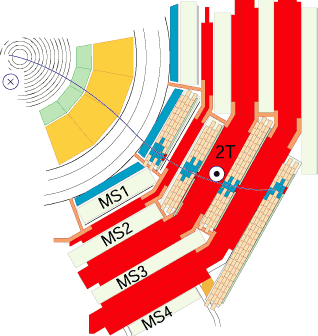
\includegraphics[width=7cm]{ll.png}
\end{center}
\caption{A muon, in the transverse plane, leaves a curved trajectory caused by magnetic field in four layers of muon detectors }
\end{figure}



\section{Triggering and Data Acquisition}

During the beam-time, almost one billion proton-proton interactions
will take place every second inside the detector. Since the number is so
huge, it is not possible to record all these data and to exactly what
we want to see and also new physics. For this reason, a trigger system was
needed in the CMS detector in order to select the potentially interesting
events and to decrease the data recorded by the computers.
\\\\
It is also known that during the collisions, even the last event have not
left the detector, new particles are generated. In order to make a clear
and precise measurement detectors must have very good resolutions and also
the electronic channels must be well synchronised. That is also a reason to the question 
why the CMS detector has a triggering system.
\\\\
The CMS detector triggering system has two level. For the Level 1
it can be said that this part of the trigger makes the work as picking
(reading) particles with large amount of energy and the ones that have unusual
particle combinations. This process is selecting the best 100.000 events
from the bilion events that we know that they happen at the CMS.
After Level 1, the Higher trigger systems collects and synchronise the
data from different parts of the detector in order to recreate the entire
event and after that it sends all these information to a computer system.
\\\\
In triggering system computers is doing the job as reading whole informations.
For their speed it can be said that they make this work in less than a 
10$^{-1}$ of a second and they help us to find for example a signature as
matching tracks to hits in the muon chambers, or spotting photons through their
high energy but lack of charge. Finally with all the process that is carried on
the triggering system, the data acquisition also provided with them in a way.

\clearpage
\section{References}
$http://cms.web.cern.ch/news/$



\end{document}
